\documentclass[submission,copyright,creativecommons]{eptcs}
%\providecommand{\event}{SOS 2007} % Name of the event you are submitting to

\usepackage{breakurl}             % Not needed if you use pdflatex only.
\usepackage{underscore}           % Only needed if you use pdflatex.
\usepackage{amssymb}
\usepackage{listings}
\usepackage{indentfirst}
\usepackage{verbatim}
\usepackage{amsmath, amsthm, amssymb}
\usepackage{graphicx}
\usepackage{url}
\usepackage{hyperref}
\usepackage{xspace}
\usepackage{placeins}

\lstdefinelanguage{scheme}{
keywords={define, conde, fresh},
sensitive=true,
%basicstyle=\small,
commentstyle=\scriptsize\rmfamily,
keywordstyle=\ttfamily\underbar,
identifierstyle=\ttfamily,
basewidth={0.5em,0.5em},
columns=fixed,
fontadjust=true,
literate={==}{{$\equiv$}}1
}

\lstdefinelanguage{ocaml}{
keywords={fresh, conde, let, begin, end, in, match, type, and, fun, function, try, with, when, class,
object, method, of, rec, repeat, until, while, not, do, done, as, val, inherit,
new, module, sig, deriving, datatype, struct, if, then, else, open, private, virtual, include, @type},
sensitive=true,
commentstyle=\small\itshape\ttfamily,
keywordstyle=\ttfamily\underbar,
identifierstyle=\ttfamily,
basewidth={0.5em,0.5em},
columns=fixed,
fontadjust=true,
literate={->}{{$\to\;\;$}}3 {===}{{$\equiv$}}3 {=/=}{{$\not\equiv$}}3 {|>}{{$\triangleright$}}3,
morecomment=[s]{(*}{*)}
}

\lstset{
mathescape=true,
identifierstyle=\ttfamily,
keywordstyle=\bfseries,
commentstyle=\scriptsize\rmfamily,
basewidth={0.5em,0.5em},
fontadjust=true,
language=ocaml
}

\sloppy

\newcommand{\miniKanren}{miniKanren\xspace}

\title{Typed Embedding of a Relational Language in OCaml}
\author{Dmitry Kosarev
\institute{Saint Petersburg State University\\ Saint Petersburg, Russia}
\email{Dmitrii.Kosarev@protonmail.ch}
\and
Dmitry Boulytchev
\institute{Saint Petersburg State University\\ Saint Petersburg, Russia}
\email{dboulytchev@math.spbu.ru}
}
\def\titlerunning{Typed Embedding of a Relational Language in OCaml}
\def\authorrunning{Dmitry Kosarev, Dmitry Boulytchev}
\begin{document}
\maketitle

\begin{abstract}
We present an implementation of the relational programming language \miniKanren as a set
of combinators and syntax extensions for OCaml. The key feature of our approach is
\emph{polymorphic unification}, which can be used to unify data structures of arbitrary types.
In addition we provide a useful generic programming pattern to systematically develop relational
specifications in a typed manner, and address the problem of integration of relational subsystems into
functional applications.
\end{abstract}

\section{Introduction}

Relational programming is an approach, based on the idea of describing programs not as functions, but 
as relations, without distinguishing between the arguments and the result value. This technique makes it 
possible to ``query'' programs in various ways, for example, to execute them ``backwards'', finding
all sets of arguments for a given result. Relational behavior can be reproduced using a number of
logic programming languages, such as Prolog, Mercury~\cite{Mercury}, 
or Curry~\cite{Curry}. 
There is also a family of embedded DSLs, specifically designed for writing declarative relational
programs that originates from \miniKanren~\cite{TRS}. \miniKanren is a minimalistic 
declarative language, initially developed for Scheme/Racket. The smallest implementation of \miniKanren 
is reported to comprise of only 40 LOC~\cite{MicroKanren,2016}; there are also more elaborate versions, including
\miniKanren with constraints~\cite{CKanren,CKanren1}, user-assisted search~\cite{Guided}, nominal unification~\cite{AlphaKanren},
etc. Due to its simplicity, \miniKanren was implemented for more than 50 other languages, such as
Haskell, Go, Smalltalk, and OCaml. In a nutshell, miniKanren introduces a minimalistic set of constructs to describe
relations over a set of syntactic terms, thus providing the same expressivity as a pure core of conventional
logic programming\footnote{A detailed miniKanren to Prolog comparison can be found at \url{http://minikanren.org/minikanren-and-prolog.html}}. 

\miniKanren has proven to be a useful tool to provide elegant solutions for various problems, otherwise considered as
non-trivial~\cite{WillThesis}. One of the most promising areas of application for \miniKanren is the implementation of
\emph{relational interpreters}. Such interpreters are capable not only to interpret programs in various directions, but also
to infer programs on the basis of expected input-output specification~\cite{Untagged}.

Being quite simple and easy to use by design, in implementation \miniKanren introduces some subtleties. Under the hood, \miniKanren 
uses a complete interleaving search~\cite{Search}. This search is guaranteed to find all existing solutions; however, it can diverge, when no 
solution exists. In reality, this amounts to divergence in a number of important cases~--- for example, when a program is asked to 
return \emph{all} existing solutions, or when the number of requested solutions exceeds the number of existing ones.
It is often possible to refactor the specification of a concrete query to avoid the divergence, but this has to be done for every execution
``direction'' of interest that compromises the idea of fully declarative relational programming.

The specifications that do not diverge even when no solutions exist, are called \emph{refutationally complete}~\cite{WillThesis}. Writing 
refutationally complete relational specifications nowadays requires knowledge of \miniKanren implementation intrinsics, and is not always
possible due to the undecidability of the fundamental computability problems. However, by developing a more advanced search it is possible
to make more specifications refutationally complete.

In this work we address one particular problem that often leads to refutational incompleteness~--- the non-commutativity of
conjunction. We present an optimization technique that is based on a certain non-termination test. Our optimization
is \emph{online} (performed during the search), \emph{non-intrusive} (does not introduce new constructs and does not require
any changes to be made to the existing specifications), and \emph{conservative} (applied only when the divergence
is detected). We prove that for the queries that return a finite number of answers, our optimization preserves convergence. 
We also demonstrate the application of the optimization for a number of interesting and important problems.

We express our gratitude to William Byrd and the reviwers of this paper for their constructive remarks and suggestions.


\section{Related Works}

\label{sec:related-works}

There are two directions of work in the process of 
incorporating negative reasoning in the logic programming:
the first considers the semantics of negation,
and the second is focused mainly on implementation aspects.

The first attempt to give a semantics 
for negation in logic programming 
was done by Clark~\cite{clark1978negation, chan1988constructive}
with his completion semantics.
It was then realized, that 
Clark's semantics has various drawbacks~\cite{van1991well}.

Przymusinski~\cite{przymusinski1989constructive} 
has studied the semantics of stratified logic programs.
He introduced the notion of \emph{perfect model semantics} for such programs.
Stratified logic programs have a variety of good properties,
including the property that each stratified program 
has a unique minimal model.

In an attempt to extend the semantics of negation
to non-stratified programs the 
\emph{well-founded semantics} was proposed~\cite{van1991well}.
However, this semantics is three-valued,
meaning that for some queries it 
can return answer \lstinline{unknown}.
For example, given the relation \lstinline{winning}
(section~\ref{sec:strat}, listing~\ref{lst:game}),
queries \lstinline{winning 'a'} and \lstinline{winning 'b'}
would return \lstinline{unknown}.

An alternative approach is 
\emph{stable model semantics}~\cite{gelfond1988stable}.
Under this semantics, non-stratified logic program
can have several stable models.
Program, that defines \lstinline{winning}, 
has two stable models, 
in one of these models goal 
\lstinline{winning 'a'} succeeds and 
\lstinline{winning 'b'} fails,
in the other \lstinline{winning 'a'} fails
and \lstinline{winning 'b'} succeeds.
Logic programming under stable model semantics
is also known under the name 
answer set programming (ASP).

The works~\cite{stuckey1991constructive, dovier2000necessary}
are theoretical studies of constructive negation
in the context of constraint logic programming.
They give a necessary and sufficient condition for the
constraint structures that are compatible with constructive negation.
Namely, the constraint structure should be \emph{admissible closed}.

From an implementation side,
Chen et al.~\cite{chen1995efficient, chen1996tabled}
developed a \textsc{Prolog} system
based on SLG resolution,
which is sound with respect to well-founded semantics.
However, they used negation as failure
with delaying of non-ground negative subgoals.
\cite{liu1999constructive} is an extension of this system
with the support of the constructive negation.
Works~\cite{bartak1998constructive, alvez2004constructive} 
implement a constraint logic programming systems
with the support of constructive negation.
Yet, as with our implementation, the
constructive negation in these systems
supports only equality and disequality
constraints over first-order terms.
We are not aware of any practical implementation 
that is parametric over arbitrary admissible closed constraint structures.

Many tools were developed to 
compute stable models of logic programs,
among them are~\cite{gebser2007clasp, giunchiglia2006answer}.
These systems usually require
to perform grounding of logic program.
The problem of finding stable models of 
ground logic program then is encoded 
as propositional formula and solved 
by some SAT solver.
Unfortunately, some logic programs
do not have finite grounding, 
but even if a program has it,
grounding may cause an exponential blow-up.
Recently, a goal-directed system
for computing stable models was developed~ 
\cite{marple2012goal, marple2017s, arias2018constraint}.
To the best of our knowledge, it is the only ASP system,
that does not require grounding.
The key components of this system are the usage of tabling, 
constructive negation, coinductive logic programming, 
and non-monotonic reasoning check.
It is an interesting and challenging task
to extend \textsc{MiniKanren} with the support of 
stable model semantics in the spirit of this line of work.

\section{\miniKanren~--- a Short Presentation}
\label{sec:demo}

In this section we briefly describe \miniKanren in its original form, using a canonical example.
\miniKanren is organized as a set of combinators and macros for Scheme/Racket, designated to describe
a search for the solution of a certain \emph{goal}. There are four domain-specific constructs
to build \emph{goals}:

\begin{itemize}
\item Syntactic unification~\cite{Unification} in the form \lstinline[language=scheme]{(== $t_1$ $t_2$)}, where $t_1$, $t_2$ are
some \emph{terms}; unification establishes a syntactic basis for all other goals. If there is a unifier for
two given terms, the goal is considered satisfied, a most general unifier is kept as a partial solution, and the execution
of current branch continues. Otherwise, the current branch backtracks.

\item Disequality constraint~\cite{CKanren} in the form \lstinline[language=scheme]{($\not\equiv$ $t_1$ $t_2$)}, where
$t_1$, $t_2$ are some terms; a disequality constraint prevents all branches (starting from the current), in which the
specified terms are equal (w.r.t. the search state), from being considered.

\item Conditional construct in the form

\begin{lstlisting}[language=scheme]
   (conde
      [$g^1_1\;\;g^1_2\;\;\dots\;\;g^1_{k_1}$]
      [$g^2_1\;\;g^2_2\;\;\dots\;\;g^2_{k_2}$]
      $\ldots$
      [$g^n_1\;\;g^n_2\;\;\dots\;\;g^n_{k_n}$]
   )
\end{lstlisting}

where each $g^i_j$ is a goal. A \lstinline{conde} goal considers each collection of subgoals, surrounded by square brackets, as
implicit conjunction (so \lstinline[language=scheme]{[$g^i_1\;\;g^i_2\;\;\dots\;\;g^i_{k_i}$] } is considered as a
conjunction of all $g^i_j$) and tries to satisfy each of them independently~--- in other words, operates on them
as a disjunction.

\item Fresh variable introduction construct in the form

\begin{lstlisting}[language=scheme]
   (fresh ($x_1\;\;x_2\;\;\dots\;\;x_k$)
     $g_1$
     $g_2$
     $\ldots$
     $g_n$
   )
\end{lstlisting}

where each $g_i$ is a goal. This form introduces fresh variables $x_1\;\;x_2\;\;\dots\;\;x_k$ and
tries to satisfy the conjunction of all subgoals $g_1\;\;g_2\;\;\dots\;\;g_n$ (these subgoals may contain
introduced fresh variables).
\end{itemize}

As an example consider a list concatenation relation; by a well-established tradition, the names
of relational objects are superscripted by ``$^o$'', hence \lstinline{append$^o$}:

\begin{lstlisting}[mathescape=true,language=scheme,numbers=left,numberstyle=\small,stepnumber=1,numbersep=-5pt]
   (define (append$^o$ x y xy)
      (conde
         [(== '() x) (== y xy)]
         [(fresh (h t ty)
            (== `(,h . ,t) x)
            (== `(,h . ,ty) xy)
            (append$^o$ t y ty))]))
\end{lstlisting}

We interpret the relation ``\lstinline{append$^o$ x y xy}'' as ``the concatenation of \lstinline{x} and \lstinline{y}
equals \lstinline{xy}''. Indeed, if the list \lstinline{x} is empty, then (regardless the content of \lstinline{y}) in order for the relation to hold
the value for \lstinline{xy} should by equal to that of \lstinline{y}~--- hence line 3. Otherwise, \lstinline{x} can be decomposed into the head
\lstinline{h} and the tail \lstinline{t}~--- so we need some fresh variables. We also need the additional variable \lstinline{ty} to designate the list
that is in the relation \lstinline{append$^o$} with \lstinline{t} and \lstinline{y}. Trivial relational reasonings complete the implementation (lines 5-7).

A goal, built with the aid of the aforementioned constructs, can be run by the following primitive:

\begin{lstlisting}[mathescape=true,language=scheme]
   run $n$ ($q_1\dots q_k$) $G$
\end{lstlisting}

Here $n$ is the number of requested answers (or ``*'' for all answers), $q_i$ are fresh query variables, and $G$ is a goal, which can
contain these variables.

The \lstinline{run} construct initiates the search for answers for a given goal and returns a (finite or infinite) list
of answers~--- the bindings for query variables, which represent individual solutions for that query. For example,

\begin{lstlisting}[mathescape=true,language=scheme]
   run 1 (q) (append$^o$ q '(3 4) '(1 2 3 4) )
\end{lstlisting}

\noindent returns a list \lstinline{((1 2))}, which constitutes the answer for query variable $q$. The process of constructing
the answers from internal data structures of miniKanren interpreter is called \emph{reification}~\cite{WillThesis}.


\section{Streams, States, and Goals}
\label{sec:goals}

This section describes a top-level framework for our implementation. Despite it contains
nothing more, than a reiteration of the original implementation~\cite{MicroKanren, CKanren}
in OCaml, we still need some notions to be properly established.

\miniKanren is organized as a set of combinators, designated to describe a search for
the solution of a certain \emph{goal}. The search itself is implemented using a
backtracking lazy stream monad:

\begin{lstlisting}
   type $\alpha$ stream

   val mplus : $\alpha$ stream -> $\alpha$ stream -> $\alpha$ stream
   val bind  : $\alpha$ stream -> ($\alpha$ -> $\beta$ stream) -> $\beta$ stream
\end{lstlisting}

Monadic primitives describe the shape of the search, and their implementations may
vary in concrete \miniKanren versions.

An essential component of the implementation is a bundle of the following types:

\begin{lstlisting}
   type env         = $\dots$
   type subst       = $\dots$
   type constraints = $\dots$

   type state = env * subst * constraints
\end{lstlisting}

Type \lstinline{state} describes a point in a lazily constructed search tree: type \lstinline{env} corresponds
to an \emph{environment}, which contains some supplementary information (in particular, environment is needed to
correctly allocate fresh variables), type \lstinline{subst} describes a substitution, which keeps current bindings
for some logical variables, and, finally, type \lstinline{constraints} represents disequality constraints,
which have to be respected. In a simplest case \lstinline{env} is just a counter for the number of the next free
variable, \lstinline{subst} is a map-like structure and \lstinline{constraints} is a list of substitutions. In our
case environment contains some extra information to make it possible to identify variables in a constant time.

The next cornerstone element is the \emph{goal} type, which is considered as a transformer of a state into
lazy stream of states:

\begin{lstlisting}
   type goal = state -> state stream
\end{lstlisting}

In terms of search, a goal nondeterministically performs one step of the search: for a given
node in a search tree it produces its immediate descendants. On the user level type \lstinline{goal}
is abstract, and states are completely hidden.

Next to last, there is a number of predefined combinators:

\begin{lstlisting}
   val (&&&)      : goal -> goal -> goal
   val (|||)      : goal -> goal -> goal
   val call_fresh : ($v$ -> goal) -> goal
   ....
\end{lstlisting}

Conjunction ``\lstinline{&&&}'' combines the results of its argument goals using \lstinline{bind},
disjunction ``\lstinline{|||}'' concatenates the results using \lstinline{mplus}, abstraction
primitive \lstinline{call_fresh} takes an abstracted goal and applies it to a freshly created
variable. Type $v$ in the latest case designates the type for a fresh variable, which we leave
abstract for now. These combinators serve as bricks for implementation of conventional
\miniKanren constructions and syntax extensions (\lstinline{conde}, \lstinline{fresh} etc.)

Finally, there are two primitive goal constructors:

\begin{lstlisting}
   val (===) : $t$ -> $t$ -> goal
   val (=/=) : $t$ -> $t$ -> goal
\end{lstlisting}

The first one is unification, while the other~--- disequality constraint. Here we, again, left
the type of terms $t$ abstract; it will be instantiated later.

In the implementation of \miniKanren both these goals are implemented using unification~\cite{CKanren}; this
is true for us as well. However, due to a drastic difference in host languages the implementation of
efficient polymorphic unification itself leads to a number of tricks with typing and data representation,
non-existing in the original version.

Described combinators allow to \emph{construct} goals. To \emph{run} a goal, the following
primitive is used:

\begin{lstlisting}
   val run : goal -> state stream
\end{lstlisting}

This primitive creates an initial state and applies a goal to it. The states in the return stream describe
various solutions for the goal. As the stream is constructed lazily, taking elements one by one makes
the search progress.

To discover concrete answers, the state has to be queried for its contents. As a rule, a few variables
are \emph{refined} in a state, i.e. their bindings in corresponding substitution are retrieved. For free
variables in addition their disequality constraints have to be \emph{reified} (e.g. represented as a list of
``forbidden'' terms). As forbidden terms can in turn contain free variables, the constraint reification
process is recursive.

In our case refinement and reification are subtle parts, since, as we will see shortly, they can not be
implemented in a type-safe part of the language.

\section{Polymorphic Unification}
\label{sec:unification}

We consider it rather natural to employ polymorphic unification in a language already equipped
with polymorphic comparison~--- a convenient, but somewhat disputable\footnote{See, for example,
\url{https://blogs.janestreet.com/the-perils-of-polymorphic-compare}} feature. Like polymorphic comparison,
polymorphic unification performs a traversal of values, exploiting intrinsic knowledge of their runtime
representation. The undeniable benefits of this solution are, first, that in order to perform unification
for user types no ``boilerplate'' code is needed, and, second, that this approach seems to deliver the
most efficient implementation. On the other hand, all the pitfalls of polymorphic comparison are inherited as
well; in particular, polymorphic unification loops for cyclic data structures and does not work for functional
values. Since we generally do not expect any reasonable outcome in these cases, the only remaining problem is that
the compiler is incapable of providing any assistance in identifying and avoiding these cases. Another drawback is that
the implementation of polymorphic unification relies on the runtime representation of values and has to be fixed
every time the representation changes.  Finally, as it is written in an unsafe manner using the \lstinline{Obj} interface,
it has to be carefully developed and tested.

An important difference between polymorphic comparison and unification is that the former only inspects its operands,
while the results of unification are recorded in a substitution (a mapping from logical variables to terms), which
later is used to reify answers. So, generally speaking, we have to show that no ill-typed
terms are constructed as a result. Overall, this property seems to be maintained vacuously, since the very
nature of (syntactic) unification is to detect whether some things can be considered equal. Nevertheless there are
different type systems and different unification implementations; in addition \emph{equal things} can be
\emph{differently typed}, so we provide here a correctness justification for a well-defined abstract case, and will
reuse this conclusion for various concrete cases.

First, we consider three alphabets:

$$
\begin{array}{rcl}
  \tau,\dots&-&\mbox{types}\\
  x^\tau,\dots&-&\mbox{typed logic variables}\\
  C_k^{\tau_1\times\tau_2\times\dots\times\tau_k\to\tau} (k\ge 0),\dots&-&\mbox{typed constructors}
\end{array}
$$

The set of all well-formed typed terms is defined by mutual induction for all types:

$$
t^\tau=x^\tau\mid C_k^{\tau_1\times\tau_2\times\dots\times\tau_k\to\tau}(t^{\tau_1},\,t^{\tau_2},\,\dots,\,t^{\tau_k})
$$

For simplicity from now on we abbreviate the notation $C_k^{\tau_1\times\tau_2\times\dots\times\tau_k\to\tau}(t^{\tau_1},\,t^{\tau_2},\,\dots,\,t^{\tau_k})$ into
$C_k^\tau(t^{\tau_1},\,t^{\tau_2},\,\dots,\,t^{\tau_k})$, keeping in mind that for any concrete constructor and for all its occurrences
in arbitrary terms all its subterms in corresponding positions agree in types.

\begin{comment}
We need also to define the notion of a subterm  $t^\tau[p]$ of a term $t^\tau$ at given position $p$:

$$
\begin{array}{rcl}
 p=\epsilon\mid\{1, 2, 3,\dots\}\bullet p&-&\mbox{the set of positions}\\
 t^\tau[\epsilon]=t^\tau&-&\mbox{base case}\\
 C_k^\tau(t_1^{\tau_1},\,t_2^{\tau_2},\dots,\,t_k^{\tau_k})[i\bullet p]=t_i^{\tau_i}[p], 1\le i \le k&-&\mbox{inductive case}
\end{array}
$$
\end{comment}

In this formulation we do not consider any structure over the set of types besides type equality, and we assume all terms are explicitly
attributed to their types at runtime. We employ this property to implement a unification algorithm in regular OCaml, using some
representation for terms and types:

\begin{lstlisting}[mathescape=true]
    val unify : term -> term -> subst option -> subst option
\end{lstlisting}

\noindent where ``\lstinline{term}'' stands for the type representing typed terms, and ``\lstinline{subst}'' stands for the type of
substitution (a partial mapping from logic variables to terms). Unification can fail (hence ``\lstinline{option}'' in the result type),
is performed in the context of existing substitution (hence ``\lstinline{subst}'' in the third argument) and can be
chained (hence ``\lstinline{option}'' in the third argument).

We use exactly the same unification algorithm with triangular substitution as in the reference implementation~\cite{MicroKanren}. We
omit here some not-so-important details (like ``occurs check'') and refrain from discussing the nature and properties of the algorithm
itself (an excellent description, including a certified correctness proof, can be found in~\cite{Kumar}).

The following snippet presents the implementation:

\begin{lstlisting}[mathescape=true,numbers=left,numberstyle=\small,stepnumber=1,numbersep=-5pt]
    let rec unify $t_1^\tau$ $t_2^\tau$ $subst$ =
      let rec walk $s$ $t^\tau$ =
        match $t^\tau$ with
        | $x^\tau$ when $x^\tau\in dom(s)$ -> $\;\;$walk $s$ $(s\;\;x^\tau)$
        | _ -> $t^\tau$
      in
      match $subst$ with
      | None -> None
      | Some $s$ ->
          match walk $s$ $t_1^\tau$, walk $s$ $t_2^\tau$ with
          | $x_1^\tau$, $x_2^\tau$ when $x_1^\tau$ = $x_2^\tau$ -> $subst$
          | $x_1^\tau$, $q_2^\tau$ -> Some ($s\;[x_1^\tau \gets q_2^\tau]$)
          | $q_1^\tau$, $x_2^\tau$ -> Some ($s\;[x_2^\tau \gets q_1^\tau]$)
          | $C^\tau(t_1^{\tau_1},\dots,t_k^{\tau_k})$, $C^\tau(p_1^{\tau_1},\dots,p_k^{\tau_k})$ ->
              unify $t_k^{\tau_k}$ $p_k^{\tau_k}$(.. (unify $t_1^{\tau_1}$ $p_1^{\tau_1}$ $subst$)$..$)
          | $\_$, $\_$ -> None
\end{lstlisting}

We remind the reader that all superscripts correspond to type attributes, which we consider here as
parts of values being manipulated. For example, line 1 means that we apply \lstinline{unify}
to terms $t_1$ and $t_2$, and expect their types to be equal $\tau$. We assume that
at the top level unification is always applied to some terms of the same type and that any
substitution can only be acquired from the empty one by a sequence of unifications.

We are going to show that under these assumptions all type attributes are superfluous~--- they
do not affect the execution of \lstinline{unify} and can be removed. Note that the only place where we
were incapable of providing an explicit type attribute was in line 4, where the result of
substitution application was returned. However, we can prove by induction that any substitution
respects the following property: if a substitution $s$ is defined for a variable $x^\tau$,
then $s\;\;x^\tau$ is attributed with the type $\tau$ (and, consequently, \lstinline{walk $s$ $t^\tau$} always
returns a term of type $\tau$).

Indeed, this property vacuously holds for the empty substitution. Let $s$ be some substitution, for which the
property holds. In the 11 we return an unchanged substitution; in line 10 we perform two calls~---
\lstinline{walk $s$ $t_1^\tau$} and \lstinline{walk $s$ $t_2^\tau$} and match their results. However,
by our induction hypothesis these results are again attributed to the type $\tau$, which justifies the
pattern matching. In line 11 we return the substitution unchanged, in lines 12 and 13 we extend the
existing substitution but preserve the property of interest. Finally, in line 15 we chain a few
applications of \lstinline{unify}; note that, again, all these calls are performed for terms of equal
types, starting from a substitution possessing the property of interest. A simple induction on the
chain length completes the proof.

So, type attributes are inessential~--- they are never analyzed and never restrict pattern matching; hence,
they can be erased completely.
We can notice now that for the representation of terms we can use OCaml's native runtime representation.
It can not be done, however, using regular OCaml~--- we have to utilize the low-level, unsafe interface \lstinline{Obj}.
Note also, we need some way to identify the occurrences of logical variables inside the terms (in the original \miniKanren
implementation the ambiguity between variable and non-variable datum representation is resolved by a convention~--- a luxury
we cannot afford).  We postpone the discussion on this subject until the next section.


%the correctness our of implementation is based on
%the following convention about logical variables: the representation of a logical variable $x^\tau$ must
%correspond to a representation of some value of type $\tau$. This, in turn, makes it somewhat problematic
%to detect a variable occurrence in a term. We postpone the discussion on this subject until Section~\ref{sec:injection}.

We call our implementation \emph{polymorphic}, since at the top level it is defined as

\begin{lstlisting}
   val unify : $\alpha$ -> $\alpha$ -> subst option -> subst option
\end{lstlisting}

The type of substitution is not polymorphic, which means that the compiler completely loses track
of types of values stored in a substitution. These types are recovered later during the reification-of-answers phase (see Section~\ref{sec:reification}).
Outside the unification the compiler maintains typing, which means that all terms, subterms, and variables agree in their types
in all contexts.

\section{Logic Variables and Injection}
\label{sec:injection}

Unification, considered in Section~\ref{sec:unification}, works for values of any types. However, it
is too generic to be used directly. As long as we use it to unify closed terms, it's ok (but rather meaningless); 
however, for terms with free variables the situation becomes more complicated. Indeed, as we've seen in the
previous section, a variable $x^\tau$ must have a runtime representation of some value of type $\tau$. As different
types may not have any values in common, if we wish to unify arbitrary types, we would need to specify the 
ground type for each logical variable explicitly, which would overthrow our implementation into a non-polymorphic 
realm with no type inference.

In this part we consider two approaches to safely handling typed terms, while preserving polymorphism and
type inference. The first is rather easy to develop and implement; unfortunately, the implementation demonstrates 
poor performance for a number of important applications. In order to fix this defficiency, we develop more 
elaborated technique, which nevertheless reuses some components from the previous one. In Section~\ref{sec:evaluation}
we present the results of performance evaluation for both approaches and compare them to that of original 
implementation.

\subsection{Tagged Logical Values}

The first natural solution is to restrict the unification to logic values only. We introduce the following polymorphic
type $[\alpha]$\footnote{In concrete syntax $\alpha\;\;$\lstinline{logic}}, which corresponds to a type, injected into
logic domain:

\begin{lstlisting}
   type $[\alpha]$ = Var of int | Value of $\alpha$
\end{lstlisting}

Note, this type cannot be disclosed to a end-user, since the only possible way to create a logic variable should 
still be by using ``\lstinline{fresh}'' construct.

Informally speaking, any value of type $[\alpha]$ is either a value of type $\alpha$, or a free
logic variable. Now, we may redefine the signature of abstraction, unification and disequality primitives in the
following manner

\begin{lstlisting}
   val call_fresh : ($[\alpha]$ -> goal) -> goal

   val (===)      : $[\alpha]$ -> $[\alpha]$ -> goal
   val (=/=)      : $[\alpha]$ -> $[\alpha]$ -> goal
\end{lstlisting}

Both unification and disequality constraint would still use the same polymorphic unification; their external, visible type,
however, is restricted to logical types only.

Apart from variables, other logical values can be obtained by injection; conversely, sometimes logical value can be projected to 
a regular one. We supply two basic functions\footnote{``\lstinline{inj}'' and ``\lstinline{prj}'' in concrete syntax.}
for these purposes

\begin{lstlisting}[mathescape=true]
   val ($\uparrow_\forall$) : $\alpha$ -> $[\alpha]$ 
   val ($\downarrow_\forall$) : $[\alpha]$ -> $\alpha$

   let ($\uparrow_\forall$) x = Value x
   let ($\downarrow_\forall$) = function Value x -> x | _ -> failwith $\mbox{``not a value''}$
\end{lstlisting}

which can be used to perform a \emph{shallow} injection/projection. As expected, the injection is total, while the projection is partial. 
Using these functions and type-specific functors, which can be derived automatically using a number of existing frameworks for 
generic programming, one can easily provide injection and projection for user-defined datatypes.

We consider user-defined list type as an example:

\begin{lstlisting}[mathescape=true]
   type ($\alpha$, $\beta$) list$_f$ = Nil | Cons of $\alpha$ * $\beta$
   
   type $\alpha$ list = ($\alpha$, $\alpha$ list) list$_f$
   type $\alpha$ list$_l$ = $[$($[\alpha]$, $\alpha$ list$_l$) list$]$

   let rec $\uparrow_{\mbox{\texttt{list}}}$ l = $\uparrow$($fmap_{\mbox{\texttt{list}}_f}$ ($\uparrow_\forall$) $\uparrow_{\mbox{\texttt{list}}}$ l) 
   let rec $\downarrow_{\mbox{\texttt{list}}}$ l = $fmap_{\mbox{\texttt{list}}_f}$ ($\downarrow_\forall$) $\downarrow_{\mbox{\texttt{list}}}$ ($\downarrow_\forall$ l)
\end{lstlisting}

Here ``\lstinline{list$_f$}'' is a custom functor for lists; note, that it is made more polymorphic, than usual~--- we abstracted it from itself 
and made it non-recursive (pragmatically speaking, it is desirable to make a type fully abstract, thus logic variables can be placed 
in arbitrary positions).

Then we provided two specialized versions~--- ``\lstinline{list}'', which corresponds to regular, non-logic lists, and ``\lstinline{list}$_l$'',
 which corresponds to logical lists with logical elements. Using a single type-specific function \lstinline{$fmap_{\mbox{\texttt{list}}_f}$}, we could easily 
provide both injection of type 

\begin{lstlisting}
   $\alpha$ list -> $\alpha$ list$_l$
\end{lstlisting} 

and projection of type 

\begin{lstlisting}
   $\alpha$ list$_l$ -> $\alpha$ list
\end{lstlisting}

Generally speaking, we can always implement injection/projection for arbitrary regular type, represented as a fixpoint of a functor~\cite{ALaCarte}, 
using only $\uparrow_\forall$, $\downarrow_\forall$ and a small set of datatype-generic combinators.

We now have to address the problem of variable identification in polymorphic unification. As we do not know the types, we cannot discriminate logical 
variables by their tags only and, thus, cannot simply use pattern matching. In our implementation we perform variable test 
as follows:

\begin{itemize}
\item in environment, we additionally keep some unique boxed value~--- \emph{anchor}~--- created by \lstinline{run} at the moment of initial
state generation; the anchor is inherited unchanged in all derived environments during the search session;
\item in each variable we additionally save the anchor, inherited from the environment, in which the variable was created;
\item inside a unification, in order to check, if we deal with a variable, we test the conjuction of the following properties:

  \begin{enumerate}
    \item the scrutenee is boxed; 
    \item the scrutenee's tag and layout correspond to those for variables;
    \item the scrutenee's anchor and current environment anchor addresses are equal.
  \end{enumerate}
\end{itemize}

Taking into account, that the state type is abstract at the user level, we guarantee, that only those variables, which were
created during current run session would pass the test, since the pointer to anchor is unique among all pointers to a boxed values 
and could not be disclosed elsewhere but in the variable creation primitive.

The only thing to describe now is the implementation of the refinement stage. The refinement is represented by the following 
function:

\begin{lstlisting}
   val refine : subst -> $[\alpha]$ -> $[\alpha]$ 
\end{lstlisting}

This function takes a substitution and a logical value and recursively substitutes all logical variables in that value w.r.t. 
the substitution until no occurrences of bound variables left. Since in our implementation the type of substitution is
not polymorphic, \lstinline{refine} is also implemented in an unsafe manner. However, it is easy to see, that \lstinline{refine} 
does not produce ill-typed terms. Indeed, all original types of variables are preserved in a substitution; unification does not 
change unified terms, so all terms, bound in a substitution, are well-typed. Hence, \lstinline{refine} always substitutes
some subterm in a well-typed term with another term of the same type, which preserves well-typedness.

In addition to performing substitutions, \lstinline{refine} also reifies disequality constrains. Reification 
attaches to each free variable in a refined term a list of \emph{refined} terms, describing the disequality constraints for that
free variable. Note, disequality can be established only for equally typed terms, which justifies type-safety of reification. 
Note also, additional care has to be taken to avoid infinite looping, since refinement and reification are
mutually recursive, and refinement of a variable can be potentially invoked from itself due to a chain of disequality 
constraints.

After refinement, the content of a logical value can be inspected via the following function:

\begin{lstlisting}
   val destruct : $[\alpha]$ -> [`Var of int * $[\alpha]$ list | `Value of $\alpha$]
\end{lstlisting}

Constructor \lstinline{`Var} corresponds to a free variable with unique integer identifier and a list of terms, 
representing all disequality constraints for this variable. These terms are refined as well.

\subsection{Untagged Logical Values and Type Bookeeping}

The solution, presented in the previous subsection, suffers from the following defficiency: in order to perform unification,
we inject terms into logic domain, making them as twice as large. As a result, this implementation loses the original one in 
terms of performance in many important applications, which compromises the very idea of using OCaml as a host language.

Here we develop an advanced version, which eliminates this penalty. As a first step, let's try to eliminate the tagging with
a drastic measure:

\begin{lstlisting}
   type $[\alpha]$ = $\alpha$
\end{lstlisting}

What consequences would this have? Of course, we would not be able to create logical variables in a conventional way. However, 
we still could have a separate type for variables

\begin{lstlisting}
   type var = Var of int * anchor
\end{lstlisting}

and use \emph{the same} variable test procedure. As the type $[\alpha]$ is abstract, this modification does not change the interface. 
As we reuse the variable test, polymorphic unification can continue work \emph{almost} correctly. The problem is that
now it can introduce the occurrences of free logic variables in non-logical, untagged, data structures. These free logic variables 
do not get in the way of unification itself (since it can handle them properly, thanks to the variable test), but they can not
be disclosed to the outer world as is.

Our idea is to use this generally unsound representation for all internal actions, and perform tagging only during the refinement
stage. However, this scenario raises the following question: what whould the type of \lstinline{refine} be? It can not be simply

\begin{lstlisting}
   val refine : subst -> $[\alpha]$ -> $[\alpha]$
\end{lstlisting}

anymore since $[\alpha]$ now equals $\alpha$. We \emph{want}, however, it be something like

\begin{lstlisting}
   val refine : subst -> $[\alpha]$ -> $(\mbox{``tagged'' }[\alpha])$
\end{lstlisting}

If $\alpha$ is not a parametric type, we can simply test, if the value is a variable, and if yes, tag it with constructor \lstinline{Var};
otherwise we tag it with \lstinline{Value}, and we're done. This trick, however, would not work for parametric types. Consider, for example, 
the refinement of a value of type \lstinline{$[[$int$]$ list$]$}. The (hypotetical) approach being described would return a value of
type \lstinline{$(\mbox{``tagged'' }[[$int$]$ list$])$}, i.e. tagged only on the top level; we need to repeat the procedure
recursively. In other words, we need the following (meta) type for the refinement primitive:

\begin{lstlisting}
   val refine : subst -> $[\alpha]$ -> $\mbox{(``tagged''} [\beta])$
\end{lstlisting}

where $\beta$ is the result of tagging $\alpha$.

These considerations can be boiled down to the following concrete implementation. 

First, we roll back to the initial definition of $[\alpha]$~--- it will play role of our ``tagged'' type.
We introduce a new, two-parametric type\footnote{In concrete syntax $(\alpha,\;\beta)\;$\lstinline{injected}.}

\begin{lstlisting}
   type $\{\alpha,\;\beta\}$ = $\alpha$
\end{lstlisting}

Of course, this type is kept abstract at the end-user level. Informally speaking, type $\{\alpha,\;\beta\}$ designates the
injection of untagged type $\alpha$ into tagged type $\beta$; the value itself is kept in the untagged form, but
tagged type can be used during the refinement stage as a constraint, which would allow to refine untagged
representation only in a feasible tagged one.

We introduce the following primivites for the type $\{\alpha,\;\beta\}$:

\begin{lstlisting}
   val lift : $\alpha$ -> $\{\alpha,\;\alpha\}$
   val inj  : $\{\alpha,\;\beta\}$ -> $\{\alpha,\;[\beta]\}$

   let lift x = x
   let inj  x = x
\end{lstlisting}

The function \lstinline{lift} puts a value into the ``bookeeping injection'' domain for the first time, while
\lstinline{inj} plays the role of bookeeping injection itself. Their composition is analogous to what was 
called ``$\uparrow_\forall$'' in the previous implementation:

\begin{lstlisting}
   val $\uparrow_\forall$ : $\alpha$ -> $\{\alpha,\;[\alpha]\}$
   let $\uparrow_\forall$ x = lift x |> inj
\end{lstlisting}

In order to deal with parametric types, we can again utilize generic programming. To handle the types with
one parameter, we introduce the following functor:

\begin{lstlisting}
   module FMap 
     (T : sig 
            type $\alpha$ t 
            val fmap : ($\alpha$ -> $\beta$) -> $\alpha$ t -> $\beta$ t 
          end
     )  : sig
            val distrib : $\{\alpha,\;\beta\}$ t -> $\{\alpha$ t, $\beta$ t$\}$
          end =
     struct
       let distrib x = x
     end
\end{lstlisting}

Note, that we do not use function ``\lstinline{T.fmap}'' in the implementation; we, however, need an inhabitant of
corresponding type to make sure we indeed deal with a functor.

In order to handle two-, three-, etc. parametric types we need higher-kinded polymorphism, which is
not supported in a direct form in OCaml. So, unfortunately, we need to introduce a separate
functors for the types with two-, three- etc. parameters; there some works on higher-kinded
polymorphism in OCaml~\cite{HKinded}, which still require the similar construction to be
erected as a bootstrap step.

Given the functor(s) of described shape, we can use it in the following manner:

\begin{lstlisting}
   module FOption = FMap 
     (struct 
        type $\alpha$ t = $\alpha$ option 
        let fmap = $fmap_{\mbox{\texttt{option}}}$ 
      end
     )

   val some : $\{\alpha, \beta\}$ -> $\{\alpha\mbox{\texttt{ option}},\;\beta\mbox{\texttt{ option}}\}$
   val none : unit  -> $\{\alpha\mbox{\texttt{ option}},\;\beta\mbox{\texttt{ option}}\}$
   
   let some x  = FOption.distrib (Some x) |> inj
   let none () = FOption.distrib None     |> inj
\end{lstlisting}

In other words, we can in a very systematic manner define \emph{logic representatives} for all constructors
of types of interest. These representatives can be used in the relational code, providing a well-bookept
typing~--- for each logical type we would be able to reconstruct its original, untagged preimage. However,
the representation of bookept types is untagged; their values are tagged only during the refinement
stage, which we can now properly type:

\begin{lstlisting}
   val refine : $\{\alpha,\;\beta\}$ -> $\beta$
\end{lstlisting}

We can implement refinement in a generic manner, adding extra functionality to the corresponding functor; we
omit the details here.

With the new implementation, the types for ``basic'' goal constructors have to be adjusted:

\begin{lstlisting}
   val (===) : $\{\alpha,\;[\beta]\}$ -> $\{\alpha,\;[\beta]\}$ -> goal
   val (=/=) : $\{\alpha,\;[\beta]\}$ -> $\{\alpha,\;[\beta]\}$ -> goal
\end{lstlisting}

As always, we require both arguments of unification and disequalify constraint to be of the same type; in addition
we require the ``injected'' part of the type to be logic.

Note, we implemented bookeeping in a completely type-safe manner, not making use of any unsafe features; in addition
we preserved polymorphism and type inference. Consider an example:

\begin{lstlisting}
   fresh (x) (x === some ($\uparrow_\forall$ 5))
\end{lstlisting}

Here the type of the term at the right hand side of unification goal is 

\begin{lstlisting}
   $\{\mbox{\texttt{int option}},\;[[\mbox{\texttt{int}}]\mbox{ \texttt{option}}]\}$
\end{lstlisting}

Hence the inferred type for the variable $x$ is the same.


\section{Reification and Top-Level Primitives}
\label{sec:reification}

In Section~\ref{sec:goals} we presented a top-level function \lstinline{run}, which
runs a goal and returns a stream of states. To acquire answers to the query,
represented by that goal, its free variables have to be reified in these states, and
we described the reification primitives in Section~\ref{sec:injection}. However,
the states keep answers in an untyped form, and the types of answers are
recovered solely on the basis of the types of variables being reified. So, the
type safety of the reification critically depends on the requirement to
reify each variable only in those states, which are descendants (w.r.t. the search tree)
of the state, in which that variable was created. In this section we describe a set of
top-level primitives, which enforce this requirement.

We provide a set of top-level combinators, which should be used to surround relational code
and perform reification in a transparent manner only in correct states.
We reimplement the top-level primitive \lstinline{run} to take three
arguments. The exact type of \lstinline{run} is rather complex and non-instructive,
so we prefer to describe the typical form of its application:

\begin{lstlisting}[mathescape=true]
   run $\overline{n}$ (fun $l_1\dots l_n$ -> $\;\;G$) (fun $a_1\dots a_n$ -> $\;\;H$)
\end{lstlisting}

Here $\overline{n}$ stands for a \emph{numeral}, which describes the number of
parameters for two other arguments of \lstinline{run}, \mbox{$l_1\dots l_n$}~---
free logical variables, $G$~--- a goal (which can make use of \mbox{$l_1\dots l_n$}),
\mbox{$a_1\dots a_n$}~--- reified answers for \mbox{$l_1\dots l_n$}, respectively, and,
finally, $H$~--- a \emph{handler} (which can make use of \mbox{$a_1\dots a_n$}).

The types of \mbox{$l_1\dots l_n$} are inferred from $G$ and always have a form

\begin{lstlisting}
   $\{\alpha,\;[\beta]\}$
\end{lstlisting}

\noindent since the types of variables can be constrained only in unification or disequality constraints.

The types of \mbox{$a_1\dots a_n$} are inferred from the types of \mbox{$l_1\dots l_n$} and
have the form

\begin{lstlisting}
   $(\alpha,\;\beta)$ reified stream
\end{lstlisting}

\noindent where the type \lstinline{reified}, in turn, is

\begin{lstlisting}
   type ($\alpha$, $\beta$) reified = $<\;$prj : $\alpha$; reify : (helper -> $\{\alpha,\;\beta\}$ -> $\beta$) -> $\beta>$
\end{lstlisting}

Two methods of this type can be used to perform two different styles of reification: first, a value without
free variables can be returned as is (using the method \lstinline{prj} which checks that in the value of
interest no free variables occur, and raises an exception otherwise). If the value contains some free
variables, it has to be properly injected into the logic domain~--- this is what \lstinline{reify} stands
for. It takes as an argument a type-specific tagging function, constructed using generic
primitives described in the previous section.

In other words a user-defined handler takes streams of reified answers for all variables supplied to the top-level
goal. All streams $a_i$ contain coherent elements, so they all have the same length and $n$-th elements of all
streams correspond to the $n$-th answer, produced by the goal $G$.

There are a few predefined numerals for one, two, etc. arguments (called, traditionally,
\lstinline{q}, \lstinline{qr}, \lstinline{qrs} etc.), and a successor function, which
can be applied to existing numeral to increment the number of expected arguments. The
implementation technique generally follows~\cite{Unparsing, DoWeNeed}.

Thus, the search and reification are tightly coupled; it is simply impossible to perform the reification
for arbitrarily-taken state and variable. This solution both guarantees the type safety and frees an end
user from the necessity to call reification primitives manually.

\section{An Example}
\label{example}

Here we present an example of relational specification, written with the aid of our library. 
For this example we take list sorting; specifically, we present sorting for lists of
natural numbers in Peano form since our library already contains built-in
support for them. However our example can be easily extended for arbitrary (but
linearly ordered) types.

List sorting can be implemented in miniKanren in a variety of ways~--- 
virtually any existing algorithm can be rewritten relationally. We, however, 
try to be as much declarative as possible to demonstrate the
advantages of relational approach. From this standpoint, we can
claim, that sorted version of empty list is empty list, and sorted version
of non-empty list is its smallest element, concatenated with sorted
version of list, containing all its remaining elements.

The following snippet literally implements this definition:

\begin{lstlisting}[mathescape=true]
   let rec sort$^o$ x y = conde [
       (x === $\uparrow$Nil) &&& (y === $\uparrow$Nil);
       fresh (s xs xs')
         (y === $\uparrow$(Cons (s, xs')))
         (sort$^o$ xs xs')       
         (smallest$^o$ x s xs)
   ]
\end{lstlisting}

The meaning of the expression

\begin{lstlisting}[mathescape=true]
   smallest$^o$ x s xs
\end{lstlisting}

is

\begin{quotation}
\noindent ``\lstinline{s}'' is the smallest element of a (non-empty) list ``\lstinline{x}'', and 
``\lstinline{xs}'' is the list of all its remaining elements.
\end{quotation}

Now, \lstinline[mathescape=true]{smallest$^o$} can be implemented
using case analysis (note, that ``\lstinline{l}'' here is a non-empty 
list):

\begin{lstlisting}[mathescape=true]
   let rec smallest$^o$ l s l' = conde [       
       (l === $\uparrow$(Cons (s, $\uparrow$Nil))) &&& (l' === $\uparrow$Nil);
       fresh (h t s' t' max)
         (l' === $\uparrow$(Cons(max,t')))
         (l === $\uparrow$(Cons(h,t)))
         (minmax$^o$ h s' s max)
         (smallest$^o$ t s' t')
   ] 
\end{lstlisting}

Finally, we implement relational minimum-maximum calculation
primitive:

\begin{lstlisting}[mathescape=true]
   let minmax$^o$ a b min max = conde [
      (min === a) &&& (max === b) &&& (le$^o$ a b);
      (max === a) &&& (min === b) &&& (gt$^o$ a b)]
\end{lstlisting}

Here ``\lstinline[mathescape=true]{le$^o$}'' and ``\lstinline[mathescape=true]{gt$^o$}'' are
built-in comparison goals for natural numbers in Peano form.

Having relational \lstinline[mathescape=true]{sort$^o$}, we can implement 
sorting for regular integer lists:

\begin{lstlisting}[mathescape=true]
   let sort l =
     run q (sorto @@ inj_nat_list l)
           (fun qs -> prj_nat_list @@ Stream.hd qs)
\end{lstlisting}

Here \lstinline{Stream.hd} is a function, which takes a head from a 
lazy stream of answers. 

It is interesting, that since \lstinline[mathescape=true]{sort$^o$} is
relational, it can be used to calculate the list of all \emph{permutations}
for a given list. Indeed, each permutation, being sorted, results in the same list. 
So, the problem of finding all permutations can be relationally reformulated into 
the problem of finding all lists, which are converted by sorting into the given one:

\begin{lstlisting}[mathescape=true]
let perm l = map prj_nat_list @@
  run q (fun q -> fresh (r)
                    (sort$^o$ (inj_nat_list l) r) 
                    (sort$^o$ q r)
        )
        (Stream.take ~n:(fact @@ length l))
\end{lstlisting}

Note, for sorting original list we used exactly the same primitive. Note also, 
we requested exactly \lstinline{fact @@ length l} answers; requesting more
would result in infinite search for non-existing answers. This concludes our example.

\section{Evaluation}
\label{sec:eval}

В данном разделе мы рассмотрим семантику с предикатом, основанном на структурной рекурсии. Также мы представим результаты апробации семантики с тремя разными предикатам на наборе примеров. Для апробации семантика была реализована на языке \textsc{Haskell} в виде интерпретатора. 


% Имперически подобранный критерий
В качестве предиката нам необходим критерий, отличающий вызов, который выгодно раскрутить сейчас от вызова, который стоит отложить. Мы предлагаем predicate by well-quasi-ordering, который эффективен для структурно-рекурсивных отношений. У таких отношений есть хотя бы один аргумент, который структурно убывает с каждым шагом рекурсии. Перестаёт убывать такой аргумент, только когда свободные переменные, которые он содержит, начинают уточняться. И когда все структурные агументы перестанут убывать, мы будем останавливать развёртку вызова.

Сначала определим отношение на кортежах термов.

\begin{definition}
Пусть $t_1^1, \ldots, t_n^1, \, t_1^2, \ldots, t_n^2 \in \mathcal{T}_{\mathcal A}$. Если для любого $i$ верно, что $height(t_i^1) \leq height(t_i^2)$, и существует $j$, для которого $height(t_i^1) < height(t_i^2)$, тогда 
\[
  (t_1^1, \ldots, t_n^1) \leq_h (t_1^2, \ldots t_n^2).
\]
\end{definition}

Отношение ``$\leq_h$'' сравнивает термы по их высоте. Оно требует, чтобы хотя бы один терм левого кордежа был строго короче, чем соответствующий терм из правого кортежа. Остальные левые термы должны быть не длиннее соотвествующих термов в правом кортеже.

\begin{lemma}
\label{lemma:wqo1}
Отношение ``$\leq_h$'' является well-quasi-ordering.
\end{lemma}
Доказывается индукцией по сумме высот всех термов.

Теперь определим отношение на парах из подстановки и реляционного применения.

\begin{definition}
Пусть $\theta_1, \theta_2$ --- подстановки,  $r_1, r_2$ --- реляционные применения. Если $r_1 = R(t^1_1,\,\ldots,\,t^1_n)$, $r_2 = R(t^2_1,\,\ldots,\,t^2_n)$, $j_1, \ldots, j_k$ --- номера структурно-рекурсивных аргументов реляционного отношения $R$ и $(\theta_1 t^1_{j_1}, \ldots, \theta_1 t^1_{j_k}) \leq_h (\theta_2 t^2_{j_1}, \ldots, \theta_2 t^2_{j_k})$, тогда
\[
  (\theta_1, r_1) \leq_{sr} (\theta_2, r_2).
\]
\end{definition}

Отношение ``$\leq_{sr}$'' сравнивает только структурно-рекурсивные аргументы двух вызовов одного отношения по высоте с помощью определенного вышe ``$\leq_h$''.

\begin{lemma}
Отношение ``$\leq_{sr}$'' является well-quasi-ordering.
\end{lemma}
Следует из леммы~\ref{lemma:wqo1}.

А значит семантика с $pred_{\leq_{sr}}$ является справедливой по теореме~\ref{todo}.

\begin{figure*}
\centering
\begin{minipage}{.5\textwidth}
  \centering
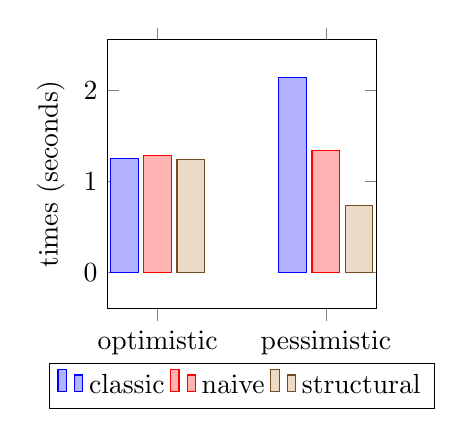
\begin{tikzpicture}
\begin{axis}[
    ybar, ymax = 2, ymin = 0.15,
    enlargelimits=0.3,
    width=5cm, height=5cm,
    legend style={at={(0.5,-0.2)},
      anchor=north,legend columns=-1},
    ylabel={times (seconds)},
    symbolic x coords={optimistic, pessimistic},
    xtick=data
    ]
\addplot coordinates {(optimistic,1.254) (pessimistic,2.142)};
\addplot coordinates {(optimistic,1.282) (pessimistic,1.337)};
\addplot coordinates {(optimistic,1.236) (pessimistic,0.733)};
\legend{classic,naive,structural}
\end{axis}
\end{tikzpicture}
 \captionof{figure}{revers$^o$ forward evaluation \\ for a list with a length of 90}
  \label{fair:plot-reverso}
\end{minipage}%
\begin{minipage}{.5\textwidth}
  \centering
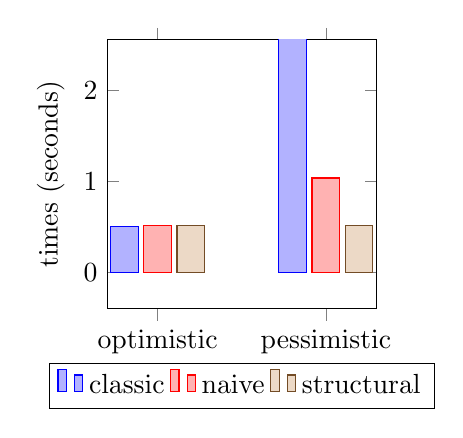
\begin{tikzpicture}
\begin{axis}[
    ybar, ymax = 2, ymin = 0.15,
    enlargelimits=0.3,
    width=5cm, height=5cm,
    legend style={at={(0.5,-0.2)},
      anchor=north,legend columns=-1},
    ylabel={times (seconds)},
    symbolic x coords={optimistic, pessimistic},
    xtick=data
    ]
\addplot coordinates {(optimistic,0.504) (pessimistic,300)};
\addplot coordinates {(optimistic,0.508) (pessimistic,1.035)};
\addplot coordinates {(optimistic,0.513) (pessimistic,0.513)};
\legend{classic,naive,structural}
\end{axis}
\end{tikzpicture}
 \captionof{figure}{sort$^o$ forward evaluation \\ for a list with a length of 5}
\label{fair:plot-sorto}
\end{minipage}
\end{figure*}

\begin{figure*}
\centering
\begin{minipage}{.5\textwidth}
  \centering
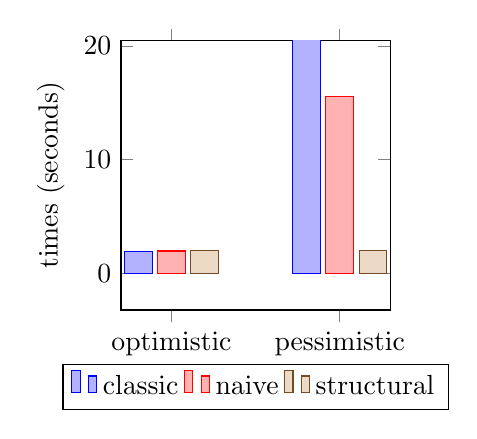
\begin{tikzpicture}
\begin{axis}[
    ybar, ymax = 16, ymin = 1.2,
    enlargelimits=0.3,
    width=5cm, height=5cm,
    legend style={at={(0.5,-0.2)},
      anchor=north,legend columns=-1},
    ylabel={times (seconds)},
    symbolic x coords={optimistic, pessimistic},
    xtick=data
    ]
\addplot coordinates {(optimistic,1.909) (pessimistic,300)};
\addplot coordinates {(optimistic,1.945) (pessimistic,15.516)};
\addplot coordinates {(optimistic,1.980) (pessimistic,1.978)};
\legend{classic,naive,structural}
\end{axis}
\end{tikzpicture}
 \captionof{figure}{``The Tower of Hanoi'' \\ solver evaluation}
\label{fair:plot-hanoi}
\end{minipage}%
\begin{minipage}{.5\textwidth}
  \centering
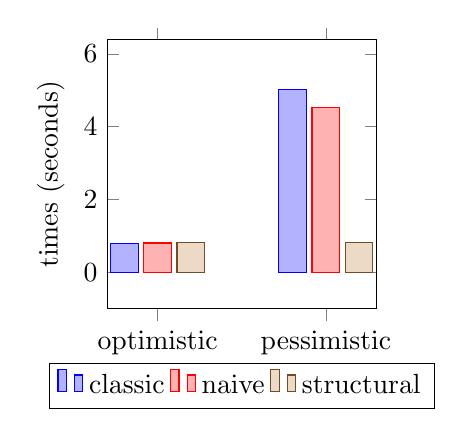
\begin{tikzpicture}
\begin{axis}[
    ybar, ymax = 5, ymin = 0.375,
    enlargelimits=0.3,
    width=5cm, height=5cm,
    legend style={at={(0.5,-0.2)},
      anchor=north,legend columns=-1},
    ylabel={times (seconds)},
    symbolic x coords={optimistic, pessimistic},
    xtick=data
    ]
\addplot coordinates {(optimistic,0.783) (pessimistic,5.019)};
\addplot coordinates {(optimistic,0.801) (pessimistic,4.522)};
\addplot coordinates {(optimistic,0.812) (pessimistic,0.817)};
\legend{classic,naive,structural}
\end{axis}
\end{tikzpicture}
 \captionof{figure}{``Bridge and torch problem'' \\ solver evaluation}
\label{fair:plot-bridge}
\end{minipage}
\end{figure*}

Now we will discuss evaluation. Целью эвалюации является выявления влияния порядка конъюнктов на эффективность трех различных семантик.

Первая семантика с предикатом $pred_{\mbox{\lstinline{true}}}$ близка к классическим реализациям \mk. В дальнейшем будем называть её {\bf left-biased}.

Вторая семантика с предикатом $pred_N$ соответсвует равномерному вычислению всех конъюнктов. Эту семантику будем назвать {\bf naive}.

Третья семантика с предикатом $pred_{\leq_{sr}}$ вычисляет структурно-рекурсивные конъюнкты, пока убывают структурно-рекурсивные аргументы. Её будем называть {\bf structural}.

For evaluation we've chosen two simple programs (list reversing and list sorting) and three more complicated (the ``Hanoi Towers''\footnote{\url{https://en.wikipedia.org/wiki/Tower_of_Hanoi}} solver, the
``Bridge and torch problem''\footnote{\url{https://en.wikipedia.org/wiki/Bridge_and_torch_problem}} solver and ``Water pouring puzzle''\footnote{\url{https://en.wikipedia.org/wiki/Water_pouring_puzzle}} solver).
% Для каждой программы мы сделали две версии. Оптимистичная версия --- это программа, в которой мы вручную подобрали оптимальный порядок конъюнктов и пессиместичная версия --- программа с неоптимальным порядком конъюнктов. В последующих диаграммах и таблице указаны средние значения 10 запусков тестов. Также для наивной равномерной конъюнкции мы подобрали количество разверток вручную. Для равномерной конъюнкции, основанной на структурной рекурсии, N было фиксировано и равно 100.
Each program was written in two versions: ``optimistic'' (with the order of important conjuncts set to provide the best performance) and ``pessimistic'' (with the order of important
conjuncts set to provide the worst performance). Also we evaluated list reversing and list sorting in both directions. In the case of the list reversing, queries \lstinline{(revers$^o$ [1;2;3] q)} and \lstinline{(revers$^o$ q [1;2;3])}\! will give the same answer \lstinline{q = [3;2;1]} but the ``optimistic'' order of conjuncts is different for them. In the case of list sorting, queries \lstinline{(sort$^o$ [1;2;3] q)} and \lstinline{(sort$^o$ q [1;2;3])} will give different answers. The first one gives sorted list \lstinline{q = [1;2;3]}, the second one gives all permutations of list \lstinline{[1;2;3]}\!\!. 

All benchmarks were run ten times, and the average time was taken. For the naive  semantics we cherry-picked the best value of unfolding bound manually. Structural arguments for each relations were detected automatically.

% На изображениях 12-15 представлены результаты апробации в виде столбцовых диаграмм. В оптимистичном случае результаты схожи для всех семантик. В пессиместичном случае время работы напрпавленной конъюнкции резко возрастает, время работы наивной равномерной конъюнкции также ворзрастает, но не так сильно. Равномерная конъюнкция, основанная на структурной рекурсии, демострирует схожую эффективность в сравнении с оптимистичным случаем.
Fig.~\ref{fair:plot-reverso}-\ref{fair:plot-bridge} show the results of evaluation in the form of bar charts. In the optimistic case, the results are similar for all semantics.
In the pessimistic case the evaluation time of the directed conjunction rapidly increases, the evaluation time of the naive fair conjunction also increases, but not so much.
The fair semantics based on structural recursion demonstrates a similar efficiency as in the optimistic case.

\begin{figure*} %[h!]
  \small
  \centering
  \begin{tabular}{ c | c | c | c | c | c | c | c }
    \multirow{2}{*}{relation} & \multirow{2}{*}{size} & 
    \multicolumn{2}{c}{left-biased semantics} &
    \multicolumn{2}{c}{naive semantics} &
    \multicolumn{2}{c}{structural semantics} \\
    \cline{3-8}
    & & optimistic & pessimistic & optimistic & pessimistic & optimistic & pessimistic  \\ 
    \hline
    \multirow{3}{*}{\begin{tabular}{c} forward \\ revers$^o$ \end{tabular}}
                 & 30   & 0.527 & 0.587  & 0.532 & 0.595   & 0.539 & 0.532 \\
                 & 60   & 0.639 & 0.947  & 0.643 & 0.790   & 0.657 & 0.577 \\
                 & 90   & 1.254 & 2.142  & 1.282 & 1.337   & 1.236 & 0.733 \\
    \hline
    \multirow{3}{*}{\begin{tabular}{c} backward \\ revers$^o$ \end{tabular}}
                 & 30   & 0.531 & 0.579  & 0.547 & 0.570  & 0.553 & 0.563 \\
                 & 60   & 0.655 & 0.875  & 0.667 & 0.812  & 0.668 & 0.681 \\
                 & 90   & 1.316 & 1.813  & 1.327 & 1.503  & 1.360 & 1.359 \\
    \hline
    \multirow{5}{*}{\begin{tabular}{c} forward \\ sort$^o$ \end{tabular}}
                 & 3    & 0.467 & 0.503  & 0.474 & 0.481  & 0.472 & 0.479 \\
                 & 4    & 0.484 & 4.679  & 0.485 & 0.493  & 0.490 & 0.488 \\
                 & 5    & 0.504 & $>$300 & 0.508 & 1.035  & 0.513 & 0.513 \\
                 & 6    & 0.526 & $>$300 & 0.237 & 14.369 & 0.544 & 0.547 \\
                 & 30   & 1.915 & $>$300 & 1.936 & $>$300 & 1.983 & 1.987 \\
    \hline
    \multirow{4}{*}{\begin{tabular}{c} backward \\ sort$^o$ \end{tabular}}
                 & 3    & 0.518 &  0.519 & 0.518 & 0.521  & 0.520 & 0.521 \\
                 & 4    & 0.533 &  0.856 & 0.534 & 0.540  & 0.534 & 0.537 \\
                 & 5    & 0.680 & 93.914 & 0.713 & 1.528  & 0.718 & 0.714 \\
                 & 6    & 2.931 & $>$300 & 2.947 & 59.647 & 2.938 & 2.936 \\
    \hline
    hanoi$^o$    & -    & 1.909 & $>$300 & 1.945 & 15.516 & 1.980 & 1.978 \\
    \hline
    bridge$^o$   & -    & 0.783 & 5.019  & 0.801 & 4.522  & 0.812 & 0.817 \\
    \hline
    water$^o$    & -    & 3.513 & $>$300 & 3.518 & $>$300 & 3.538 & 3.771

  \end{tabular}
  \caption{The results of evaluation: running times of benchmarks in seconds}
  \label{fair:evaluation-table}
\end{figure*}

% Более подробно результаты представлены на изображении 16. Можно заметить, что время работы программы sorto в пессиместичном случае очень быстро растет с увеличением длины списка для направленной конъюнкции и наивной равномерной. В случае с равномерной конъюнкцией, основанной на структурной рекурсии, пессиместичный случай растет сопостовимо с оптимистичным.
The results are presented in more detail in Fig.~\ref{fair:evaluation-table}. ``Hanoi Towers'' solver has name \lstinline{hanoi$^o$}, ``Bridge and torch problem'' solver has name \lstinline{bridge$^o$} and ``Water pouring puzzle'' solver has name \lstinline{water$^o$}. We can conclude that forward and backward \lstinline{sort$^o$} runtime in the pessimistic case increases very rapidly with increasing the list length for left-biased and naive fair semantics. In the case of the fair semantics based on structural recursion the running time in pessimistic case increases on a par with that in the optimistic one. Also the solver \lstinline{water$^o$} very slow in the pessimistic case for left-biased and naive fair. However, fair conjunction based on structural recursion pessimistic case is no different from an optimistic case.


% Подводя итог, равномерная конъюнкция, основанная на структурной рекурсии сопоставима по эффективности с направленной конъюнкцией. Более того, это конъюнкция слабо зависит от порядка конъюнктов.
To summarize, the fair semantics based on structural recursion does not introduce any essential overhead in comparison with left-biased semantics in an optimistic case. At the same time it
weakly depends on the order of the conjuncts, and thus demonstrates much better performance in the pessimistic case.

\section{Conclusion}
\label{conclusion}

We presented an approach for converting typed functional programs into relations. Relational conversion 
in many cases allows us to avoid tedious recoding of functional specifications into relational form and to 
concentrate on writing relational specifications only when their reconstruction from functions is impossible or 
undesirable. Our implementation works for the subset of OCaml; we evaluated it for a number of interesting 
examples and acquired some new relational solutions.

There is a number of directions for future research. First, a performance evaluation is desirable~--- at
present time we do not know, what slowdown factor is. Another problem is a development of an approach to
prove complete correctness (or refute this claim).


\nocite{*}
\bibliographystyle{eptcs}
\bibliography{ocanren}

\end{document}
